\documentclass[]{article}
\usepackage{lmodern}
\usepackage{amssymb,amsmath}
\usepackage{ifxetex,ifluatex}
\usepackage{fixltx2e} % provides \textsubscript
\ifnum 0\ifxetex 1\fi\ifluatex 1\fi=0 % if pdftex
  \usepackage[T1]{fontenc}
  \usepackage[utf8]{inputenc}
\else % if luatex or xelatex
  \ifxetex
    \usepackage{mathspec}
  \else
    \usepackage{fontspec}
  \fi
  \defaultfontfeatures{Ligatures=TeX,Scale=MatchLowercase}
\fi
% use upquote if available, for straight quotes in verbatim environments
\IfFileExists{upquote.sty}{\usepackage{upquote}}{}
% use microtype if available
\IfFileExists{microtype.sty}{%
\usepackage{microtype}
\UseMicrotypeSet[protrusion]{basicmath} % disable protrusion for tt fonts
}{}
\usepackage[margin = 1.5in]{geometry}
\usepackage{hyperref}
\PassOptionsToPackage{usenames,dvipsnames}{color} % color is loaded by hyperref
\hypersetup{unicode=true,
            pdftitle={Introduction to ggplot},
            pdfauthor={Abhinav Anand},
            colorlinks=true,
            linkcolor=blue,
            citecolor=magenta,
            urlcolor=red,
            breaklinks=true}
\urlstyle{same}  % don't use monospace font for urls
\usepackage{color}
\usepackage{fancyvrb}
\newcommand{\VerbBar}{|}
\newcommand{\VERB}{\Verb[commandchars=\\\{\}]}
\DefineVerbatimEnvironment{Highlighting}{Verbatim}{commandchars=\\\{\}}
% Add ',fontsize=\small' for more characters per line
\usepackage{framed}
\definecolor{shadecolor}{RGB}{248,248,248}
\newenvironment{Shaded}{\begin{snugshade}}{\end{snugshade}}
\newcommand{\KeywordTok}[1]{\textcolor[rgb]{0.13,0.29,0.53}{\textbf{#1}}}
\newcommand{\DataTypeTok}[1]{\textcolor[rgb]{0.13,0.29,0.53}{#1}}
\newcommand{\DecValTok}[1]{\textcolor[rgb]{0.00,0.00,0.81}{#1}}
\newcommand{\BaseNTok}[1]{\textcolor[rgb]{0.00,0.00,0.81}{#1}}
\newcommand{\FloatTok}[1]{\textcolor[rgb]{0.00,0.00,0.81}{#1}}
\newcommand{\ConstantTok}[1]{\textcolor[rgb]{0.00,0.00,0.00}{#1}}
\newcommand{\CharTok}[1]{\textcolor[rgb]{0.31,0.60,0.02}{#1}}
\newcommand{\SpecialCharTok}[1]{\textcolor[rgb]{0.00,0.00,0.00}{#1}}
\newcommand{\StringTok}[1]{\textcolor[rgb]{0.31,0.60,0.02}{#1}}
\newcommand{\VerbatimStringTok}[1]{\textcolor[rgb]{0.31,0.60,0.02}{#1}}
\newcommand{\SpecialStringTok}[1]{\textcolor[rgb]{0.31,0.60,0.02}{#1}}
\newcommand{\ImportTok}[1]{#1}
\newcommand{\CommentTok}[1]{\textcolor[rgb]{0.56,0.35,0.01}{\textit{#1}}}
\newcommand{\DocumentationTok}[1]{\textcolor[rgb]{0.56,0.35,0.01}{\textbf{\textit{#1}}}}
\newcommand{\AnnotationTok}[1]{\textcolor[rgb]{0.56,0.35,0.01}{\textbf{\textit{#1}}}}
\newcommand{\CommentVarTok}[1]{\textcolor[rgb]{0.56,0.35,0.01}{\textbf{\textit{#1}}}}
\newcommand{\OtherTok}[1]{\textcolor[rgb]{0.56,0.35,0.01}{#1}}
\newcommand{\FunctionTok}[1]{\textcolor[rgb]{0.00,0.00,0.00}{#1}}
\newcommand{\VariableTok}[1]{\textcolor[rgb]{0.00,0.00,0.00}{#1}}
\newcommand{\ControlFlowTok}[1]{\textcolor[rgb]{0.13,0.29,0.53}{\textbf{#1}}}
\newcommand{\OperatorTok}[1]{\textcolor[rgb]{0.81,0.36,0.00}{\textbf{#1}}}
\newcommand{\BuiltInTok}[1]{#1}
\newcommand{\ExtensionTok}[1]{#1}
\newcommand{\PreprocessorTok}[1]{\textcolor[rgb]{0.56,0.35,0.01}{\textit{#1}}}
\newcommand{\AttributeTok}[1]{\textcolor[rgb]{0.77,0.63,0.00}{#1}}
\newcommand{\RegionMarkerTok}[1]{#1}
\newcommand{\InformationTok}[1]{\textcolor[rgb]{0.56,0.35,0.01}{\textbf{\textit{#1}}}}
\newcommand{\WarningTok}[1]{\textcolor[rgb]{0.56,0.35,0.01}{\textbf{\textit{#1}}}}
\newcommand{\AlertTok}[1]{\textcolor[rgb]{0.94,0.16,0.16}{#1}}
\newcommand{\ErrorTok}[1]{\textcolor[rgb]{0.64,0.00,0.00}{\textbf{#1}}}
\newcommand{\NormalTok}[1]{#1}
\usepackage{graphicx,grffile}
\makeatletter
\def\maxwidth{\ifdim\Gin@nat@width>\linewidth\linewidth\else\Gin@nat@width\fi}
\def\maxheight{\ifdim\Gin@nat@height>\textheight\textheight\else\Gin@nat@height\fi}
\makeatother
% Scale images if necessary, so that they will not overflow the page
% margins by default, and it is still possible to overwrite the defaults
% using explicit options in \includegraphics[width, height, ...]{}
\setkeys{Gin}{width=\maxwidth,height=\maxheight,keepaspectratio}
\IfFileExists{parskip.sty}{%
\usepackage{parskip}
}{% else
\setlength{\parindent}{0pt}
\setlength{\parskip}{6pt plus 2pt minus 1pt}
}
\setlength{\emergencystretch}{3em}  % prevent overfull lines
\providecommand{\tightlist}{%
  \setlength{\itemsep}{0pt}\setlength{\parskip}{0pt}}
\setcounter{secnumdepth}{0}
% Redefines (sub)paragraphs to behave more like sections
\ifx\paragraph\undefined\else
\let\oldparagraph\paragraph
\renewcommand{\paragraph}[1]{\oldparagraph{#1}\mbox{}}
\fi
\ifx\subparagraph\undefined\else
\let\oldsubparagraph\subparagraph
\renewcommand{\subparagraph}[1]{\oldsubparagraph{#1}\mbox{}}
\fi

%%% Use protect on footnotes to avoid problems with footnotes in titles
\let\rmarkdownfootnote\footnote%
\def\footnote{\protect\rmarkdownfootnote}

%%% Change title format to be more compact
\usepackage{titling}

% Create subtitle command for use in maketitle
\newcommand{\subtitle}[1]{
  \posttitle{
    \begin{center}\large#1\end{center}
    }
}

\setlength{\droptitle}{-2em}
  \title{Introduction to ggplot}
  \pretitle{\vspace{\droptitle}\centering\huge}
  \posttitle{\par}
  \author{Abhinav Anand}
  \preauthor{\centering\large\emph}
  \postauthor{\par}
  \date{}
  \predate{}\postdate{}

\linespread{1.3}

\begin{document}
\maketitle

\section{Setup}\label{setup}

The following discussion assumes you have donwloaded R and RStudio.
Additionally, the package suite \texttt{tidyverse()} which includes the
package \texttt{ggplot2()} needs to be included.

\begin{enumerate}
\def\labelenumi{\arabic{enumi}.}
\tightlist
\item
  For downloading R, visit \url{https://cran.r-project.org/}
\item
  For downloading RStudio visit \url{https://www.rstudio.com/}
\item
  For downloading \texttt{ggplot2()}, type
  \texttt{install.packages("ggplot2")} or equivalently for
  \texttt{tidyverse()} type \texttt{install.packages("tidyverse")}
\end{enumerate}

\section{Introduction to ggplot}\label{introduction-to-ggplot}

The \texttt{gg} of \texttt{ggplot} stands for (layered)
\texttt{grammar\ of\ graphics} (Wilkinson 2005), (Wickham 2010). This
idea will be further explored by the means of data from the package
\texttt{gapminder()}. To install, type
\texttt{install.packages("gapminder")} in the RStudio console.

\begin{Shaded}
\begin{Highlighting}[]
\NormalTok{data_gapminder <-}\StringTok{ }\NormalTok{gapminder}\OperatorTok{::}\NormalTok{gapminder }
\end{Highlighting}
\end{Shaded}

\subsection{Notes}\label{notes}

\begin{enumerate}
\def\labelenumi{\arabic{enumi}.}
\item
  Why \texttt{\textless{}-} as opposed to \texttt{=} ?
\item
  Why \texttt{gapminder::gapminder} ?
\item
  What is a dataframe?
\end{enumerate}

A data frame is a rectangular collection of variables (in the columns)
and observations (in the rows). It's different from a `mere' matrix
since the columns have variable names usually.

\subsection{Questions?}\label{questions}

\subsubsection{\texorpdfstring{Are ``Western'' countries richer than
``Eastern''
countries?}{Are Western countries richer than Eastern countries?}}\label{are-western-countries-richer-than-eastern-countries}

The current state of Europe (in 2007):

\begin{Shaded}
\begin{Highlighting}[]
\NormalTok{data_eur_}\DecValTok{2007}\NormalTok{ <-}\StringTok{ }\NormalTok{data_gapminder }\OperatorTok\StringTok{ }
\StringTok{  }\NormalTok{dplyr}\OperatorTok{::}\KeywordTok{filter}\NormalTok{(year }\OperatorTok{==}\StringTok{ }\DecValTok{2007}\NormalTok{) }\OperatorTok\StringTok{ }\CommentTok{#isolates variables for year 2007}
\StringTok{  }\NormalTok{dplyr}\OperatorTok{::}\KeywordTok{filter}\NormalTok{(continent }\OperatorTok{==}\StringTok{ "Europe"}\NormalTok{) }

\NormalTok{plot_eur <-}\StringTok{ }\KeywordTok{ggplot}\NormalTok{(}\DataTypeTok{data =}\NormalTok{ data_eur_}\DecValTok{2007}\NormalTok{) }\OperatorTok{+}
\StringTok{  }\KeywordTok{geom_point}\NormalTok{(}\DataTypeTok{mapping =} \KeywordTok{aes}\NormalTok{(}\DataTypeTok{x =}\NormalTok{ gdpPercap, }\DataTypeTok{y =}\NormalTok{ country)) }

\NormalTok{plot_eur}
\end{Highlighting}
\end{Shaded}

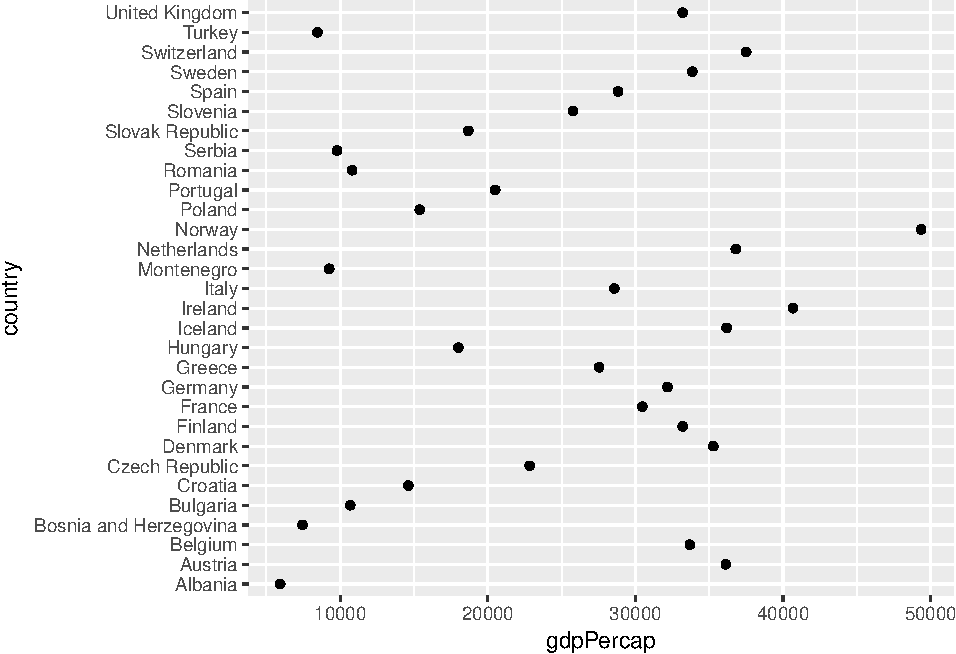
\includegraphics{Intro_ggplot_files/figure-latex/plot_eur-1.pdf}

There is high variation---from Albania to Norway.

What about Asian countries in 2007?

\begin{Shaded}
\begin{Highlighting}[]
\NormalTok{data_asia_}\DecValTok{2007}\NormalTok{ <-}\StringTok{ }\NormalTok{data_gapminder }\OperatorTok\StringTok{ }
\StringTok{  }\NormalTok{dplyr}\OperatorTok{::}\KeywordTok{filter}\NormalTok{(year }\OperatorTok{==}\StringTok{ }\DecValTok{2007}\NormalTok{) }\OperatorTok\StringTok{ }\CommentTok{#isolates variables for year 2007}
\StringTok{  }\NormalTok{dplyr}\OperatorTok{::}\KeywordTok{filter}\NormalTok{(continent }\OperatorTok{==}\StringTok{ "Asia"}\NormalTok{) }\CommentTok{#collect only Asian countries}

\NormalTok{plot_asia <-}\StringTok{ }\KeywordTok{ggplot}\NormalTok{(}\DataTypeTok{data =}\NormalTok{ data_asia_}\DecValTok{2007}\NormalTok{) }\OperatorTok{+}
\StringTok{  }\KeywordTok{geom_point}\NormalTok{(}\DataTypeTok{mapping =} \KeywordTok{aes}\NormalTok{(}\DataTypeTok{x =}\NormalTok{ gdpPercap, }\DataTypeTok{y =}\NormalTok{ country)) }\OperatorTok{+}
\StringTok{  }\KeywordTok{labs}\NormalTok{(}\DataTypeTok{x =} \StringTok{"GDP/capita (USD)"}\NormalTok{, }
       \DataTypeTok{y =} \StringTok{"Country"}\NormalTok{,}
       \DataTypeTok{title =} \StringTok{"GDP per capita in Asia"}\NormalTok{,}
       \DataTypeTok{subtitle =} \StringTok{"Measured in USD (2007)"}\NormalTok{)}

\NormalTok{plot_asia}
\end{Highlighting}
\end{Shaded}

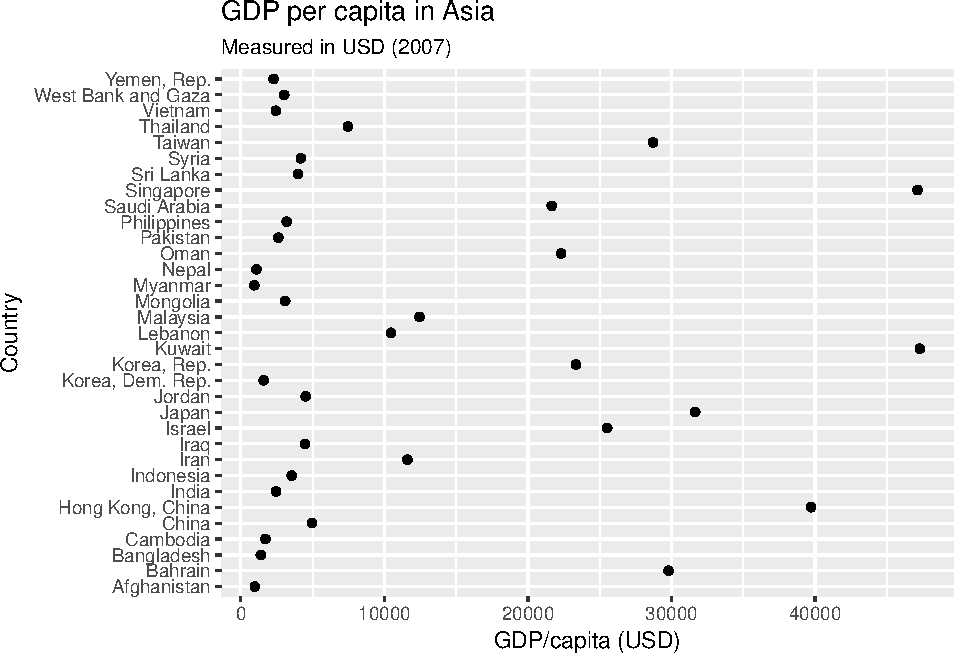
\includegraphics{Intro_ggplot_files/figure-latex/plot_asia-1.pdf}

Again, large variation among Asian countries but what about the bounds?
What can we say about the question?

\subsection{Graphics}\label{graphics}

We start with the function \texttt{ggplot()}. It creates a coordinate
system that we will add layers to. The first argument is the dataset to
use in the graph.

\texttt{ggplot(data\ =\ data\_eur\_2007)} creates an empty graph. The
function \texttt{geom\_point()} adds a layer of points to our plot. Each
geom function in ggplot2 takes a mapping argument. This defines how
variables in our dataset are mapped to aesthetics such as axes, colors,
shapes etc. The \(x\) and \(y\) arguments of \texttt{aes()} specify
which variables to map to the \(x\) and \(y\) axes. Variables can also
be mapped to aesthetics such as colors, shapes, size etc.

\subsubsection{A More Granular Look: China, India, France,
Germany}\label{a-more-granular-look-china-india-france-germany}

\begin{Shaded}
\begin{Highlighting}[]
\NormalTok{data_CIFU <-}\StringTok{ }\NormalTok{data_gapminder }\OperatorTok
\StringTok{  }\NormalTok{dplyr}\OperatorTok{::}\KeywordTok{filter}\NormalTok{(country }\OperatorTok\StringTok{ }\KeywordTok{c}\NormalTok{(}\StringTok{"China"}\NormalTok{, }\StringTok{"India"}\NormalTok{, }\StringTok{"France"}\NormalTok{, }\StringTok{"Germany"}\NormalTok{))}

\NormalTok{(plot_CIFU_life_exp <-}\StringTok{ }\KeywordTok{ggplot}\NormalTok{(}\DataTypeTok{data =}\NormalTok{ data_CIFU) }\OperatorTok{+}
\StringTok{  }\KeywordTok{geom_line}\NormalTok{(}\DataTypeTok{mapping =} \KeywordTok{aes}\NormalTok{(}\DataTypeTok{x =}\NormalTok{ year, }\DataTypeTok{y =}\NormalTok{ lifeExp, }\DataTypeTok{color =}\NormalTok{ country))}
\NormalTok{  )}
\end{Highlighting}
\end{Shaded}

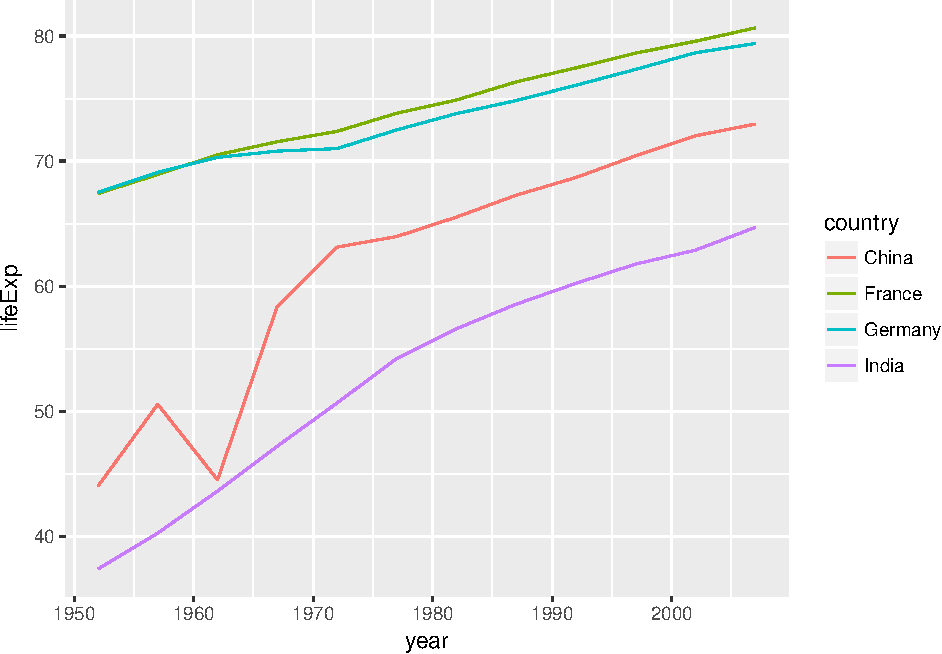
\includegraphics{Intro_ggplot_files/figure-latex/CIFU-1.pdf}

\subsubsection{Notes}\label{notes-1}

\begin{enumerate}
\def\labelenumi{\arabic{enumi}.}
\tightlist
\item
  Plots can be stored as variables too.
\item
  Other aesthetic attributes: shape, size, alpha (transparency) etc.
\item
  Note where to put the \texttt{+} sign.
\item
  \texttt{geom\_line()} as opposed to points. Other ``geoms'' are
  \texttt{geom\_smooth}, \texttt{geom\_boxplot}, \texttt{geom\_bar} etc.
\end{enumerate}

\subsubsection{Faceting}\label{faceting}

\begin{Shaded}
\begin{Highlighting}[]
\NormalTok{(plot_CIFU_life_cont <-}\StringTok{ }\KeywordTok{ggplot}\NormalTok{(}\DataTypeTok{data =}\NormalTok{ data_CIFU) }\OperatorTok{+}
\StringTok{  }\KeywordTok{geom_line}\NormalTok{(}\DataTypeTok{mapping =} \KeywordTok{aes}\NormalTok{(}\DataTypeTok{x =}\NormalTok{ year, }\DataTypeTok{y =}\NormalTok{ lifeExp, }\DataTypeTok{color =}\NormalTok{ country)) }\OperatorTok{+}
\StringTok{  }\KeywordTok{facet_wrap}\NormalTok{(}\OperatorTok{~}\StringTok{ }\NormalTok{continent)}
\NormalTok{ )}
\end{Highlighting}
\end{Shaded}

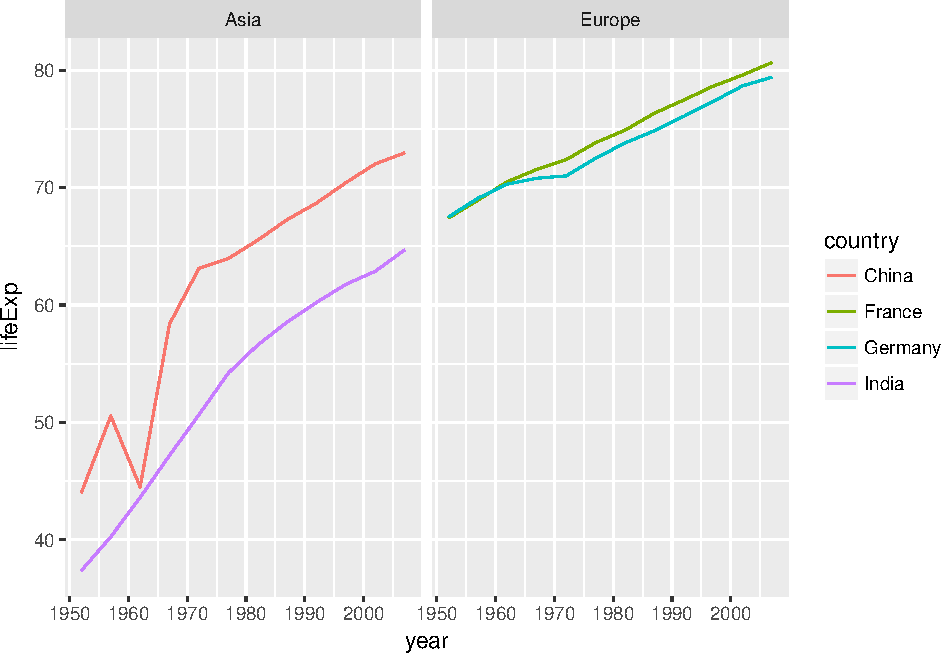
\includegraphics{Intro_ggplot_files/figure-latex/CIFU_Facet-1.pdf}

\subsubsection{Notes}\label{notes-2}

\begin{enumerate}
\def\labelenumi{\arabic{enumi}.}
\tightlist
\item
  To facet on one variable (`continent' here), use
  \texttt{facet\_wrap()}.
\item
  To facet on two variables, use \texttt{facet\_grid()}
\end{enumerate}

\subsection{\texorpdfstring{Geoms in
\texttt{ggplot()}}{Geoms in ggplot()}}\label{geoms-in-ggplot}

REWRITE:

A geom is the geometrical object that a plot uses to represent data.
People often describe plots by the type of geom that the plot uses. For
example, bar charts use bar geoms, line charts use line geoms, boxplots
use boxplot geoms, and so on. Scatterplots break the trend; they use the
point geom. As we see above, you can use different geoms to plot the
same data.

However, not every aesthetic works with every geom. You could set the
shape of a point, but you couldn't set the ``shape'' of a line. On the
other hand, you could set the linetype of a line. Multiple geoms could
be part of the same graph. ggplot2 provides over 30 geoms

To display multiple geoms in the same plot, add multiple geom functions
to ggplot():

ggplot(data = mpg) + geom\_point(mapping = aes(x = displ, y = hwy)) +
geom\_smooth(mapping = aes(x = displ, y = hwy))

This, however, introduces some duplication in our code. Imagine if you
wanted to change the y-axis to display cty instead of hwy. You'd need to
change the variable in two places, and you might forget to update one.
You can avoid this type of repetition by passing a set of mappings to
ggplot(). ggplot2 will treat these mappings as global mappings that
apply to each geom in the graph. In other words, this code will produce
the same plot as the previous code:

ggplot(data = mpg, mapping = aes(x = displ, y = hwy)) + geom\_point() +
geom\_smooth()

\subsection{Bar Charts}\label{bar-charts}

\subsection{Boxplots}\label{boxplots}

\texttt{coord\_flip()}

p2 \textless{}- ggplot(housing, aes(x = Home.Value)) p2 +
geom\_histogram()

\texttt{themes()}: Built-in themes include:

theme\_gray() (default) theme\_bw() theme\_classc()s

\subsection{The Main FAQ}\label{the-main-faq}

\subsection{Wide Versus Long Data}\label{wide-versus-long-data}

\section*{References}\label{references}
\addcontentsline{toc}{section}{References}

\hypertarget{refs}{}
\hypertarget{ref-Wickham:2010}{}
Wickham, Hadley. 2010. ``A Layered Grammar of Graphics.'' \emph{Journal
of Computational and Graphical Statistics} 19 (1): 3--28.

\hypertarget{ref-Wilkinson:2005}{}
Wilkinson, Leland. 2005. \emph{The Grammar of Graphics (Statistics and
Computing)}. Berlin, Heidelberg: Springer-Verlag.


\end{document}
